% !TEX encoding = UTF-8
% !TEX program = xelatex
% !TEX spellcheck = en_US

\documentclass[degree=master,degree-type=academic,fontset=windows]{gzuthesis}
  % 学位 degree:
  %   doctor | master
  % 学位类型 degree-type:
  %   academic（默认）| professional
  % 字体库 fontset
  %   windows | mac | fandol | ubuntu
  % 建议终版使用 Windows 平台的字体编译


% 论文基本配置，加载宏包等全局配置
% !TEX root = ./gzuthesis-example.tex

% 论文基本信息配置

\gzusetup{
  %******************************
  % 注意：
  %   1. 配置里面不要出现空行
  %   2. 不需要的配置信息可以删除
  %   3. 建议先阅读文档中所有关于选项的说明
  %******************************
  %
  % 输出格式
  %   选择打印版（print）或用于提交的电子版（electronic），前者会插入空白页以便直接双面打印
  %
  output = electronic,
  %
  % 标题
  %   可使用“\\”命令手动控制换行
  %
  title  = {贵州大学学位论文 \LaTeX{} 模板},
  title* = {An Introduction to \LaTeX{} Thesis Template of \\ Guizhou
            University v\version},
  %
  % 学科门类
  %   1. 学术型
  %      - 中文
  %        需注明所属的学科门类，例如：
  %        哲学、经济学、法学、教育学、文学、历史学、理学、工学、农学、医学、
  %        军事学、管理学、艺术学
  %      - 英文
  %        博士：Doctor of Philosophy
  %        硕士：
  %          哲学、文学、历史学、法学、教育学、艺术学门类，公共管理学科
  %          填写“Master of Arts“，其它填写“Master of Science”
  %   2. 专业型
  %      直接填写专业学位的名称，例如：
  %      教育博士、工程硕士等
  %      Doctor of Education, Master of Engineering
  %
  degree-category  = {工学硕士},
  degree-category* = {Master of Science},
  %
  % 培养单位
  %   填写所属院系的全名
  %
  department = {计算机科学与技术系},
  %
  % 学科
  %   1. 研究生学术型学位，获得一级学科授权的学科填写一级学科名称，其他填写二级学科名称
  %   2. 本科生填写专业名称，第二学位论文需标注“（第二学位）”
  %
  discipline  = {电子信息},
  discipline* = {Electronic Information},
  research-direction = {大数据技术与工程},
  research-direction* = {Big Data Technology and Engineering},
  %
  % 专业领域
  %   1. 设置专业领域的专业学位类别，填写相应专业领域名称
  %   2. 2019 级及之前工程硕士学位论文，在 `engineering-field` 填写相应工程领域名称
  %   3. 其他专业学位类别的学位论文无需此信息
  %
  % professional-field  = {计算机技术},
  % professional-field* = {Computer Technology},
  %
  % 姓名
  %
  author     = {王小华},
  author*    = {Wang Xiaohua},
  student-id = {2024025084},
  %
  % 学号
  % 仅当书写开题报告时需要（同时设置 `thesis-type = proposal'）
  %
  % student-id = {2000310000},
  %
  % 指导教师
  %   中文姓名和职称之间以英文逗号“,”分开，下同
  %
  supervisor  = {张安思, 副教授},
  supervisor* = {Professor Zhang Ansi},
  %
  % 副指导教师
  %
%   associate-supervisor  = {陈文光, 教授},
%   associate-supervisor* = {Professor Chen Wenguang},
  %
  % 联合指导教师
  %
  % co-supervisor  = {某某某, 教授},
  % co-supervisor* = {Professor Mou Moumou},
  %
  % 日期
  %   使用 ISO 格式；默认为当前时间
  %
  date            = {2027-06-01},
  graduation-year = {2027},
  %
  % 是否在中文封面后的空白页生成书脊（默认 false）
  %
  include-spine = false,
  %
  % 密级和年限
  %   秘密, 机密, 绝密
  %
  secret-level = {公开},
  % secret-year  = {10},
  %
  % 封面
  clc                = {TP999},
  udc                = {2024025084},
  school-code        = {10657},
}

% 载入所需的宏包

% 定理类环境宏包
\usepackage{amsthm}
% 也可以使用 ntheorem
% \usepackage[amsmath,thmmarks,hyperref]{ntheorem}

\gzusetup{
  %
  % 数学字体
  math-style = ISO,  % GB | ISO | TeX
  math-font  = xits  % stix | xits | libertinus
}

% 可以使用 nomencl 生成符号和缩略语说明
% \usepackage{nomencl}
% \makenomenclature

% 表格加脚注
\usepackage{threeparttable}

% 表格中支持跨行
% \usepackage{multirow}

% 固定宽度的表格。
% \usepackage{tabularx}

% 跨页表格
\usepackage{longtable}

% 算法
\usepackage{algorithm}
\usepackage{algorithmic}

% 量和单位
\usepackage{siunitx}

% 参考文献使用 BibTeX + natbib 宏包
% 顺序编码制
% \usepackage[sort]{natbib}
% \bibliographystyle{gzuthesis-numeric}
% 使用 BibTeX + natbib
% \usepackage[sort]{natbib}
% \bibliographystyle{plainnat}

% GB/T 7714—2025 参考文献格式
% 顺序编码制
\usepackage[sort]{gbt7714}

% 贵州大学要求参考文献表列出全部作者
\gbtsetup{
  maxbibnames = 0,
  minbibnames = 0,
  inline      = true,
}

\bibliographystyle{gbt7714-2025-numeric}


% 著者-出版年制
% \usepackage{natbib}
% \bibliographystyle{gzuthesis-author-year}


% 本科生参考文献的著录格式
% \usepackage[sort]{natbib}
% \bibliographystyle{gzuthesis-bachelor}

% 参考文献使用 BibLaTeX 宏包
% \usepackage[style=gzuthesis-numeric]{biblatex}
% \usepackage[style=gzuthesis-author-year]{biblatex}
% \usepackage[style=gzuthesis-bachelor]{biblatex}
% \usepackage[style=apa]{biblatex}
% \usepackage[style=mla-new]{biblatex}

% 声明 BibLaTeX 的数据库
% \addbibresource{ref/refs.bib}

% 定义所有的图片文件在 figures 子目录下
\graphicspath{{figures/}}

% 数学命令
% \newcommand\dif{\mathop{}\!\mathrm{d}}
\makeatletter
\newcommand\dif{%
  \mathop{}\!%
  \ifgzu@math@style@TeX
    d%
  \else
    \mathrm{d}%
  \fi
}
\makeatother

% hyperref 宏包在最后调用
\usepackage{hyperref}


\begin{document}

% 封面
\maketitle

% 学位论文指导小组、公开评阅人和答辩委员会名单
% % 参数	默认值	控制内容
% body-width	0.86\textwidth	整个红框内的信息区域宽度
% line-height	24bp	正文信息的基线间距
% row-sep	2mm	委员、秘书、时间、地点之间的附加间距
% role-width	4\ccwd	右侧主席/委员的预留宽度
% role-gap	0.5\ccwd	下划线终点与角色之间的距离
% name-align	column	姓名采用统一中心线还是逐条居中, line
% name-position	0.63	统一姓名中心线距信息区域左端的比例，仅 column 模式使用



% 模式	行为
% name-align=column（默认）	所有姓名的中心在同一竖直线上，适合你提供的 Word 样式
% name-align=line	每个姓名严格位于自己所在横线的正中，但不同姓名可能不在同一竖直线上

%
% name-align = column,
% name-position = 0.65,
% 表示所有姓名的中心位置设在信息区域宽度的 65% 处，姓名整体比默认位置略靠右。所有名字仍然处在同一竖直线上。




\begin{committee}[
  name = {硕士学位论文答辩委员会名单},
  body-width = 0.8\textwidth,
  line-height = 34bp,
  row-sep = 0mm,
  name-align = column,
  name-position = 0.63,
  role-gap = 0.5\ccwd
]

\committeemember{XXXX大学XXX教授}{xxx}{主席}
\committeemember{XXXX大学XXX教授}{xxx}{委员}
\committeemember{贵州大学教授/博导}{xxx}{委员}
\committeemember{贵州大学教授/博导}{xxx}{委员}

\committeesecretary[
  before-name = 1\ccwd,
  before-title = 1\ccwd
]{XXX}{副教授/博士研究生}

\committeedate{XXXX年XX月XX日}
\committeeplace{贵州大学西校区崇厚楼XXXX}

\end{committee}



% 也可以导入 Word 版转的 PDF 文件
% \begin{committee}[file=figures/committee.pdf]
% \end{committee}

% 使用授权的说明
% \copyrightpage
% 将签字扫描后授权文件 scan-copyright.pdf 替换原始页面
% \copyrightpage[file=scan-copyright.pdf]

\frontmatter
\begin{abstractzh}
学位论文的规范排版是准确表达研究内容和组织学术材料的重要基础。本示例围绕贵州大学硕士学位论文的编排要求，展示从题名页、答辩委员会名单和声明页，到中英文摘要、目次、正文及结尾部分的完整组织方式。文档中的姓名、学号、单位及研究内容均为示例，使用时需要由作者据实替换。

模板将论文基本信息集中设置，统一生成前置页面，并分别控制正文、章节标题、图表题注和参考文献的字体与字号。针对中文论文中常见的长网址、多行表格、跨页公式和附录编号问题，示例给出了可直接使用的写法。正文后的致谢、参考文献、附录、索引、作者简历和后记采用独立的样式，同时保持页码连续。

本摘要仅说明模板的用途，不报告任何实际科研发现。正式撰写时，中文摘要应概括研究目的、方法、结果和结论，突出研究工作的创新或改进，通常控制在三百至一千字，并选择三至八个关键词。英文摘要应与中文摘要的内容对应。作者应在提交前逐项核对论文信息、声明签名、参考文献及院系补充要求。
\end{abstractzh}

\begin{abstracten}
Consistent thesis formatting supports the clear presentation of research and the organization of academic material. This example demonstrates the structure of a master's thesis at Guizhou University, from the title page, defense committee and declarations to the Chinese and English abstracts, contents, main text and end matter. Names, student details, affiliations and research descriptions are illustrative and must be replaced with accurate information.

The template stores thesis information centrally and generates the preliminary pages with consistent fonts and sizes. Examples address long URLs, multiline table cells, equations spanning pages and appendix numbering. Acknowledgements, references, appendices, an index, the author's curriculum vitae and a postscript have separate styles while retaining continuous page numbers.

This abstract describes the template and reports no research findings. In an actual thesis, the abstract should state the research purpose, methods, results and conclusions, with emphasis on the contributions or improvements. The Chinese abstract normally contains 300 to 1,000 Chinese characters and three to eight keywords. The English abstract should convey the same content. Authors should verify all personal information, declaration signatures, references and additional departmental requirements before submission.
\end{abstracten}


% 目录
\tableofcontents

% 插图和附表清单
\listoffigures           % 插图清单
\listoftables            % 附表清单
% \listoffiguresandtables  % 插图和附表清单

% 符号对照表
% !TEX root = ../gzuthesis-example.tex

\begin{denotation}[3cm]
  \item[PI] 聚酰亚胺
  \item[MPI] 聚酰亚胺模型化合物，N-苯基邻苯酰亚胺
  \item[PBI] 聚苯并咪唑
  \item[MPBI] 聚苯并咪唑模型化合物，N-苯基苯并咪唑
  \item[PY] 聚吡咙
  \item[PMDA-BDA] 均苯四酸二酐与联苯四胺合成的聚吡咙薄膜
  \item[MPY] 聚吡咙模型化合物
  \item[As-PPT] 聚苯基不对称三嗪
  \item[MAsPPT] 聚苯基不对称三嗪单模型化合物，3,5,6-三苯基-1,2,4-三嗪
  \item[DMAsPPT] 聚苯基不对称三嗪双模型化合物（水解实验模型化合物）
  \item[S-PPT] 聚苯基对称三嗪
  \item[MSPPT] 聚苯基对称三嗪模型化合物，2,4,6-三苯基-1,3,5-三嗪
  \item[PPQ] 聚苯基喹噁啉
  \item[MPPQ] 聚苯基喹噁啉模型化合物，3,4-二苯基苯并二嗪
  \item[HMPI] 聚酰亚胺模型化合物的质子化产物
  \item[HMPY] 聚吡咙模型化合物的质子化产物
  \item[HMPBI] 聚苯并咪唑模型化合物的质子化产物
  \item[HMAsPPT] 聚苯基不对称三嗪模型化合物的质子化产物
  \item[HMSPPT] 聚苯基对称三嗪模型化合物的质子化产物
  \item[HMPPQ] 聚苯基喹噁啉模型化合物的质子化产物
  \item[PDT] 热分解温度
  \item[HPLC] 高效液相色谱（High Performance Liquid Chromatography）
  \item[HPCE] 高效毛细管电泳色谱（High Performance Capillary lectrophoresis）
  \item[LC-MS] 液相色谱-质谱联用（Liquid chromatography-Mass Spectrum）
  \item[TIC] 总离子浓度（Total Ion Content）
  \item[\textit{ab initio}] 基于第一原理的量子化学计算方法，常称从头算法
  \item[DFT] 密度泛函理论（Density Functional Theory）
  \item[$E_a$] 化学反应的活化能（Activation Energy）
  \item[ZPE] 零点振动能（Zero Vibration Energy）
  \item[PES] 势能面（Potential Energy Surface）
  \item[TS] 过渡态（Transition State）
  \item[TST] 过渡态理论（Transition State Theory）
  \item[$\increment G^\neq$] 活化自由能（Activation Free Energy）
  \item[$\kappa$] 传输系数（Transmission Coefficient）
  \item[IRC] 内禀反应坐标（Intrinsic Reaction Coordinates）
  \item[$\nu_i$] 虚频（Imaginary Frequency）
  \item[ONIOM] 分层算法（Our own N-layered Integrated molecular Orbital and molecular Mechanics）
  \item[SCF] 自洽场（Self-Consistent Field）
  \item[SCRF] 自洽反应场（Self-Consistent Reaction Field）
\end{denotation}



% 也可以使用 nomencl 宏包，需要在导言区
% \usepackage{nomencl}
% \makenomenclature

% 在这里输出符号说明
% \printnomenclature[3cm]

% 在正文中的任意为都可以标题
% \nomenclature{PI}{聚酰亚胺}
% \nomenclature{MPI}{聚酰亚胺模型化合物，N-苯基邻苯酰亚胺}
% \nomenclature{PBI}{聚苯并咪唑}
% \nomenclature{MPBI}{聚苯并咪唑模型化合物，N-苯基苯并咪唑}
% \nomenclature{PY}{聚吡咙}
% \nomenclature{PMDA-BDA}{均苯四酸二酐与联苯四胺合成的聚吡咙薄膜}
% \nomenclature{MPY}{聚吡咙模型化合物}
% \nomenclature{As-PPT}{聚苯基不对称三嗪}
% \nomenclature{MAsPPT}{聚苯基不对称三嗪单模型化合物，3,5,6-三苯基-1,2,4-三嗪}
% \nomenclature{DMAsPPT}{聚苯基不对称三嗪双模型化合物（水解实验模型化合物）}
% \nomenclature{S-PPT}{聚苯基对称三嗪}
% \nomenclature{MSPPT}{聚苯基对称三嗪模型化合物，2,4,6-三苯基-1,3,5-三嗪}
% \nomenclature{PPQ}{聚苯基喹噁啉}
% \nomenclature{MPPQ}{聚苯基喹噁啉模型化合物，3,4-二苯基苯并二嗪}
% \nomenclature{HMPI}{聚酰亚胺模型化合物的质子化产物}
% \nomenclature{HMPY}{聚吡咙模型化合物的质子化产物}
% \nomenclature{HMPBI}{聚苯并咪唑模型化合物的质子化产物}
% \nomenclature{HMAsPPT}{聚苯基不对称三嗪模型化合物的质子化产物}
% \nomenclature{HMSPPT}{聚苯基对称三嗪模型化合物的质子化产物}
% \nomenclature{HMPPQ}{聚苯基喹噁啉模型化合物的质子化产物}
% \nomenclature{PDT}{热分解温度}
% \nomenclature{HPLC}{高效液相色谱（High Performance Liquid Chromatography）}
% \nomenclature{HPCE}{高效毛细管电泳色谱（High Performance Capillary lectrophoresis）}
% \nomenclature{LC-MS}{液相色谱-质谱联用（Liquid chromatography-Mass Spectrum）}
% \nomenclature{TIC}{总离子浓度（Total Ion Content）}
% \nomenclature{\textit{ab initio}}{基于第一原理的量子化学计算方法，常称从头算法}
% \nomenclature{DFT}{密度泛函理论（Density Functional Theory）}
% \nomenclature{$E_a$}{化学反应的活化能（Activation Energy）}
% \nomenclature{ZPE}{零点振动能（Zero Vibration Energy）}
% \nomenclature{PES}{势能面（Potential Energy Surface）}
% \nomenclature{TS}{过渡态（Transition State）}
% \nomenclature{TST}{过渡态理论（Transition State Theory）}
% \nomenclature{$\increment G^\neq$}{活化自由能（Activation Free Energy）}
% \nomenclature{$\kappa$}{传输系数（Transmission Coefficient）}
% \nomenclature{IRC}{内禀反应坐标（Intrinsic Reaction Coordinates）}
% \nomenclature{$\nu_i$}{虚频（Imaginary Frequency）}
% \nomenclature{ONIOM}{分层算法（Our own N-layered Integrated molecular Orbital and molecular Mechanics）}
% \nomenclature{SCF}{自洽场（Self-Consistent Field）}
% \nomenclature{SCRF}{自洽反应场（Self-Consistent Reaction Field）}


% 正文部分
\mainmatter
\chapter{绪论}\label{chap:intro}
\section{研究背景与问题提出}
异常检测关注不符合预期行为的观测或模式。相关研究在统计假设、异常定义和
应用约束上存在差异，不能仅凭一个分数阈值统一解释所有场景\cite{chandola2009survey}。
本例将无人机飞行记录抽象为多变量时间序列：每个架次由同步采集的多个变量组成，
不同架次之间则保留独立的起止边界。这样的表示便于讨论时序依赖、变量关联与部署流程。

对于同一时刻的观测，高残差既可能反映异常，也可能来自模型未学习到的正常机动。
因此，论文中的问题描述应区分观测空间、模型假设和决策规则。
本例关注的问题不是“用复杂模型得到更高分数”，而是怎样把数据划分、预测、
阈值校准和指标计算组成一条清晰可复查的链路。

\subsection{示例目标与边界}
本文具有两个相互区分的目标。第一，给出可执行的小型时序异常检测流程；
第二，提供覆盖学位论文常见元素的排版样本。两者通过统一的数据文件和自动生成的
结果表连接，但不能相互替代。模板编译成功并不意味着模型有效，
合成数据上得到有限的检测效果也不意味着模板满足所有学校规范。

示例没有调用真实无人机数据集，也没有实现神经网络预训练。
“飞行”“传感器”“故障”等词在实验部分描述的是合成信号的设计角色。
所给出的方法为透明基线，最终结论限于该脚本和指定参数。
这一约束也适用于封面、摘要与英文摘要中的表述。

\subsection{工程组织原则}
论文源码按章节拆分，实验数据与图表由脚本生成，参考文献统一维护在一个数据库中。
正文不手写“图 3-1”或“式（4-2）”等会随编辑失效的编号，而使用标签和交叉引用。
所有浮动体的题注先于标签写入，使引用指向相应对象，而不是此前的章节计数器。

\section{相关研究概述}
\subsection{序列预测与表示学习}
长短期记忆网络通过门控结构处理序列中的信息传递问题\cite{hochreiter1997lstm}。
Transformer 则以注意力机制组织序列表示\cite{vaswani2017attention}。
这些方法提供了不同的建模工具，但模型结构与异常判据不是同一概念。
将预测器用于异常检测时，仍需定义残差聚合、训练数据范围及阈值来源。

\citet{nie2023patchtst} 通过分块输入和通道独立设计研究时间序列预测。
\citet{zeng2023dlinear} 则以简单线性模型检验一组预测基准上的结构选择。
这些研究说明，比较对象应与具体任务和实验协议对应；
本例选择岭回归只是为了降低复现门槛，不是用未经运行的神经网络结果充当对照。

\subsection{异常判据与通用时序模型}
Deep SVDD 研究在特征空间中约束正常样本表示的方法\cite{ruff2018deep}。
Anomaly Transformer 通过关联差异构造时序异常判据\cite{xu2022anomaly}。
MOMENT 将多个时序任务纳入预训练模型框架\cite{goswami2024moment}。
本例在综述中引用这些工作，但实验中不报告它们的性能，
也不将自己的合成数据分数与其论文中的公开结果直接排序。

\subsection{软件工具与复现}
机器学习基础概念可参见周志华的教材\cite{zhou2016ml}，
深度学习中的表示、优化与正则化讨论可参见 Goodfellow 等人的专著\cite{goodfellow2016deep}。
在工具层面，scikit-learn 提供了多种机器学习算法接口\cite{pedregosa2011sklearn}，
PyOD 将不同异常检测方法组织在统一工具箱中\cite{zhao2019pyod}。
本工程的数值脚本只依赖 NumPy 与 Matplotlib，不要求读者安装上述完整工具箱。

\section{本文内容与章节安排}
第~\ref{chap:foundations}~章定义时序窗口、异常分数及评价指标；
第~\ref{chap:data}~章说明合成数据和架次级划分；
第~\ref{chap:method}~章给出岭回归、平滑和阈值校准；
第~\ref{chap:experiments}~章报告自动生成的结果并讨论局限；
第~\ref{chap:conclusions}~章总结案例与后续工作。
附录~\ref{app:config}、附录~\ref{app:proof} 和附录~\ref{app:reproduce}
分别提供配置字典、补充推导与复现清单。

本节同时展示三种引用写法：普通引用\cite{chandola2009survey}、
行内引用\ExampleInlineCite{vaswani2017attention}，以及
\citet{goswami2024moment} 形式的叙述引用。
参考文献后端的切换只影响著录和引用格式，不改变章节内容。

\chapter{基础理论与问题定义}\label{chap:foundations}
\section{多变量序列与滑动窗口}
设第 $k$ 个架次的观测为
$\mat{X}^{(k)}=[\vect{x}^{(k)}_0,\ldots,\vect{x}^{(k)}_{T_k-1}]^{\mathsf T}$，
其中 $\vect{x}^{(k)}_t\in\Rset^C$。本例采用零起始下标，与 Python 数组索引一致。
一个长度为 $L$ 的窗口只包含待预测时刻之前的观测：
\begin{equation}
 \mat{U}^{(k)}_t=
 \begin{bmatrix}
 (\vect{z}^{(k)}_{t-L})^{\mathsf T}\\
 (\vect{z}^{(k)}_{t-L+1})^{\mathsf T}\\
 \vdots\\
 (\vect{z}^{(k)}_{t-1})^{\mathsf T}
 \end{bmatrix}\in\Rset^{L\times C},\qquad t=L,\ldots,T_k-1.
 \label{eq:window}
\end{equation}
式~\eqref{eq:window} 同时演示了矩阵换行和行内维度说明。
窗口顺序展平后构成 $LC$ 维向量，附加常数项得到
$\vect{u}_t\in\Rset^{LC+1}$。样本输入中不含 $\vect{z}_t$，
因此这种组织方式可以用于一步因果预测。

\begin{definition}[合法的架次内窗口]\label{def:window}
若窗口中所有输入观测和目标观测均属于同一个架次，且输入时刻严格小于目标时刻，
则称该窗口为合法的架次内预测窗口。
\end{definition}

\begin{proposition}[窗口数量]\label{prop:count}
对于长度为 $T$ 的架次，在窗口长度为 $L$、步长为 1、预测长度为 1 且
$T>L$ 的条件下，可生成 $T-L$ 个合法窗口。
\end{proposition}
\begin{proof}
合法目标时刻从 $L$ 到 $T-1$，其整数个数为
$(T-1)-L+1=T-L$。每个目标时刻唯一对应此前的 $L$ 个观测，故结论成立。
\end{proof}

\section{数据标准化与尺度}
对于各变量的不同量纲，仅使用训练数据估计均值和标准差。
令 $\mathcal{T}$ 为训练观测集合，则
\begin{align}
 \mu_c &= \frac{1}{|\mathcal{T}|}\sum_{(k,t)\in\mathcal{T}}x^{(k)}_{t,c},\label{eq:mu}\\
 \sigma_c &= \sqrt{\frac{1}{|\mathcal{T}|}\sum_{(k,t)\in\mathcal{T}}
       (x^{(k)}_{t,c}-\mu_c)^2},\label{eq:std}\\
 z^{(k)}_{t,c} &= \frac{x^{(k)}_{t,c}-\mu_c}{\max(\sigma_c,\varepsilon)}.
 \label{eq:normalize}
\end{align}
本例取 $\varepsilon=10^{-8}$。训练和标准化公式中的分母均使用总体形式，
与脚本的 \texttt{ddof=0} 保持一致。校准集与测试集不重新拟合这两个统计量。

\section{异常分数与决策}
\subsection{残差分数}
预测器输出 $\widehat{\vect{z}}_t$ 后，将各通道的平方误差平均：
\begin{equation}
 e_t=\frac{1}{C}\sum_{c=1}^{C}(z_{t,c}-\widehat z_{t,c})^2.
 \label{eq:residual}
\end{equation}
该分数位于标准化空间，是非负标量。它不是概率，因而不应直接解释为
“系统发生故障的概率”。对所有通道取平均还意味着不同变量拥有相同聚合权重，
这种选择在真实应用中需要结合传感器噪声和安全重要性重新评估。

\subsection{阈值与二值标签}
给定平滑分数 $s_t$ 和阈值 $\tau$，预测标签为
\begin{equation}
 \widehat y_t=
 \begin{cases}
 1,&s_t>\tau,\\
 0,&s_t\leq\tau.
 \end{cases}\label{eq:decision}
\end{equation}
异常分数较高并不自动意味着模型已经定位故障部件。
本例只报告异常点判断，不把通道误差大小等同于因果解释。

\section{评价指标与实现约定}
在对应窗口目标的测试时刻计算 TP、FP、TN 和 FN；每个架次的前 $L$ 个点
没有对应预测，因而不计入评价。精确率、召回率、F1 和误报率分别为
\begin{align}
 P&=\frac{\mathrm{TP}}{\mathrm{TP}+\mathrm{FP}},&
 R&=\frac{\mathrm{TP}}{\mathrm{TP}+\mathrm{FN}},\\
 F_1&=\frac{2PR}{P+R},&
 \mathrm{FAR}&=\frac{\mathrm{FP}}{\mathrm{FP}+\mathrm{TN}}.
 \label{eq:metrics}
\end{align}
当分母为零时，脚本将相应的精确率、召回率或 F1 设为零。
AUROC 则由正负样本分数的排序计算，并对并列分数采用平均秩。
本例始终使用逐点标签，不以命中异常区间中的一个点替换整段预测。

上述约定使数字结果可以追溯到明确的程序行为。
但是，逐点指标不能完整描述报警延迟和重复报警成本。
这些工程属性应在真实任务中单独报告，而不应通过修改逐点标签隐式表达。

\chapter{合成数据与实验协议}\label{chap:data}
\DemoNotice
\section{变量设计与生成过程}
本例使用六个通道代表姿态、运动状态和动力相关观测。
每个架次包含 1000 个点，采样间隔为 \qty{0.05}{\second}，
时间戳范围为 \qtyrange{0}{49.95}{\second}。
表~\ref{tab:channels} 给出字段定义。名称只是便于理解的物理类比，
生成器没有实现空气动力学或飞控方程，也不能用于验证飞行安全。

\begin{table}[htbp]
\centering
\gzucaption{合成数据的通道定义}{Channel definitions of the synthetic data}
\label{tab:channels}
\begin{tabularx}{\textwidth}{@{}cllX@{}}
\toprule
编号 & 字段 & 单位 & 合成角色 \\
\midrule
1 & \texttt{roll\_deg} & 度 & 周期横滚与随机扰动 \\
2 & \texttt{pitch\_deg} & 度 & 俯仰周期项与横滚耦合 \\
3 & \texttt{airspeed\_mps} & m/s & 基础空速与横滚相关项 \\
4 & \texttt{altitude\_m} & m & 缓变高度与俯仰相关项 \\
5 & \texttt{throttle} & 无量纲 & 周期控制量与小幅噪声 \\
6 & \texttt{current\_a} & A & 与控制量关联的电流观测 \\
\bottomrule
\end{tabularx}
\end{table}

以横滚通道为例，第 $k$ 个架次的基础信号为
\begin{equation}
 x^{(k)}_{t,1}=6\sin(2\pi\cdot0.08\,t\Delta t+\phi_k)
       +0.8\sin(2\pi\cdot0.5\,t\Delta t)+\epsilon^{(k)}_{t,1},
 \label{eq:generator}
\end{equation}
其中 $\Delta t=0.05$，$\phi_k$ 为架次特定的相位，噪声标准差为 0.10。
其他变量含有不同频率的周期项和显式的线性耦合项。
所有随机数来自确定的种子规则，完整表达式以附带 Python 源码为准。

\begin{figure}[htbp]
\centering
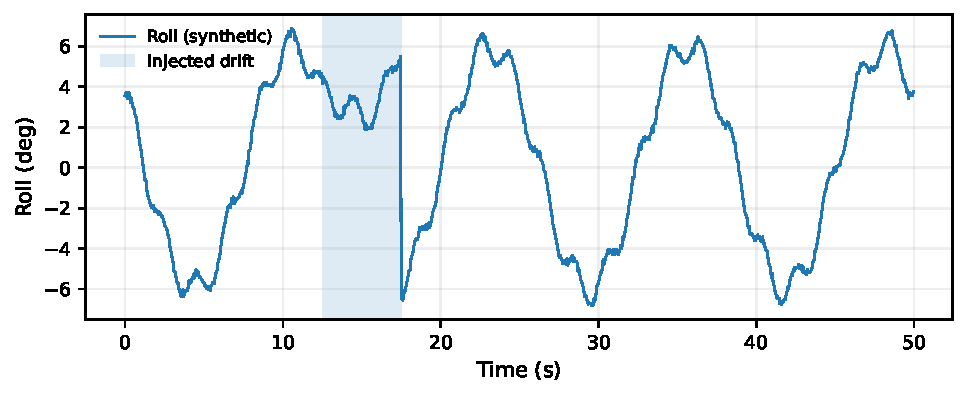
\includegraphics[width=.94\textwidth]{roll-series.pdf}
\gzucaption[合成横滚信号]{第 F10 架次的合成横滚信号与注入漂移区间}
 {Synthetic roll signal and injected drift interval in flight F10}
\label{fig:roll}
\end{figure}

图~\ref{fig:roll} 展示了正常周期项与人为注入的漂移。
图中的横坐标使用秒，异常区间由生成器记录，不由检测结果反推。
这一区分保证真实标签在评估时保持独立。

\section{异常注入规则}
三个测试架次采用相同的区间定义，但基础相位和噪声不同。
所有区间都使用左闭右开的数组约定，见表~\ref{tab:events}。
这种约定与 Python 切片完全一致，避免边界点的重复标记。

\begin{table}[htbp]
\centering
\gzucaption{仅在测试集注入的合成异常}{Synthetic anomalies injected only into test flights}
\label{tab:events}
\begin{tabularx}{\textwidth}{@{}lccX@{}}
\toprule
类型 & 索引区间 & 通道 & 具体操作 \\
\midrule
渐变漂移 & $[250,350)$ & 横滚 & 叠加从 0 到 12 的线性增量 \\
高频振动 & $[520,600)$ & 俯仰 & 叠加幅值 3、频率 5 Hz 的正弦项 \\
恒定偏置 & $[700,780)$ & 电流 & 在基础观测上增加 3 A \\
\bottomrule
\end{tabularx}
\end{table}

正常生成过程没有复杂的传感器饱和、通信丢包、控制回路响应和飞行包线约束。
因此，异常可能比真实故障更规则，也可能与真实机动的统计特征不同。
本文报告这些限制，而不把合成异常描述为经过试飞验证的故障模式。

\section{架次级数据划分}
训练集为 F01--F06，校准集为 F07--F09，测试集为 F10--F12。
表~\ref{tab:split} 给出观测数和有效窗口数。
划分在滑窗前完成，每个架次内部再独立构造窗口。

\begin{table}[htbp]
\centering
\gzucaption{架次级划分与有效窗口数量}{Flight-level splits and valid window counts}
\label{tab:split}
\begin{tabular}{@{}llrrl@{}}
\toprule
子集 & 架次 & 原始点数 & 窗口数 & 用途 \\
\midrule
训练 & F01--F06 & 6000 & \DemoTrainWindows & 标准化与拟合 \\
校准 & F07--F09 & 3000 & \DemoCalWindows & 阈值估计 \\
测试 & F10--F12 & 3000 & \DemoTestWindows & 最终评价 \\
\bottomrule
\end{tabular}
\end{table}

每个架次使用 $L=9$，有效窗口数由命题~\ref{prop:count} 得到。
训练架次的数组可以在统计均值时拼接，但不能在拼接后直接跨边界滑窗。
二者虽然都出现了“拼接”，数学对象却不同：前者计算无序汇总统计，
后者会人为制造本不存在的连续时序上下文。

\section{校准与测试的隔离}
模型超参数和分位数在运行前给定，本例没有利用测试 F1 选择阈值。
改变平滑系数时，重新对校准分数计算阈值，而不是沿用另一组分数尺度的阈值。
测试标签仅在所有分数和阈值确定后进入指标函数。
这条数据依赖关系在算法~\ref{alg:pipeline} 中进一步展开。

为便于复查，原始合成观测保存为 CSV，统计量和配置保存为 JSON，
结果行保存为可直接输入的 LaTeX 片段。正文中的关键统计数字通过宏读取，
重新运行脚本后即可同步更新，避免表格已经变化但摘要仍保留旧数字。

\chapter{预测残差检测流程}\label{chap:method}
\section{总体结构}
图~\ref{fig:pipeline} 展示本例的处理流程。
训练数据用于拟合预测器，正常校准数据用于估计阈值，测试数据仅通过固定流程输出结果。
图中箭头表示数据依赖而非真实飞控系统中的控制指令。

\begin{figure}[htbp]
\centering
\begin{tikzpicture}[
  box/.style={draw,align=center,minimum width=30mm,minimum height=13mm,
    font=\fontsize{10bp}{13bp}\selectfont,inner sep=3pt},
  arr/.style={-{Stealth[length=2mm]},semithick},
  node distance=10mm and 8mm]
\node[box] (train) {训练架次\\标准化统计};
\node[box,right=of train] (window) {架次内滑窗\\$L=9$};
\node[box,right=of window] (model) {岭回归预测\\固定参数};
\node[box,right=of model] (score) {残差与平滑\\$e_t\rightarrow s_t$};
\node[box,below=of model] (cal) {正常校准集\\分位数阈值 $\tau$};
\node[box,below=of score] (out) {测试判断\\$s_t>\tau$};
\draw[arr] (train)--(window);
\draw[arr] (window)--(model);
\draw[arr] (model)--(score);
\draw[arr] (score)--(out);
\draw[arr] (cal)--(out);
\end{tikzpicture}
\gzucaption{示例方法的数据处理流程}{Processing pipeline of the demonstration method}
\label{fig:pipeline}
\end{figure}

\section{线性预测与正则化}
\subsection{模型定义}
将 $N$ 个训练窗口堆叠为 $\mat{A}\in\Rset^{N\times(LC+1)}$，
对应目标组成 $\mat{Y}\in\Rset^{N\times C}$。
模型参数为 $\mat{W}\in\Rset^{(LC+1)\times C}$，
预测满足 $\widehat{\mat{Y}}=\mat{A}\mat{W}$。
常数列对应截距项，训练目标为
\begin{equation}
 \min_{\mat{W}}\ \|\mat{A}\mat{W}-\mat{Y}\|_{\mathrm F}^{2}
     +\lambda\operatorname{tr}(\mat{W}^{\mathsf T}\mat{D}\mat{W}),
 \quad\mat{D}=\diag(1,\ldots,1,0).
 \label{eq:ridge-objective}
\end{equation}
最后一个对角元素为零，表示不惩罚截距。
本例使用残差平方和而不是残差均方作为优化目标，因此 $\lambda=1$
的含义应与具体目标函数一同报告。

\subsection{求解形式与数值实现}
对应正规方程为
\begin{equation}
 (\mat{A}^{\mathsf T}\mat{A}+\lambda\mat{D})\mat{W}
 =\mat{A}^{\mathsf T}\mat{Y}.
 \label{eq:normal-equation}
\end{equation}
实现使用线性方程求解器，不显式计算矩阵逆。
附录~\ref{app:proof} 给出唯一性条件及推导。
这里的矩阵列数只有 $LC+1=55$，便于在普通 CPU 环境下复现。
这不是对大规模神经模型训练成本的估计。

\begin{assumption}[训练设计矩阵条件]\label{ass:ridge}
至少存在一个训练窗口，$\lambda>0$，并且设计矩阵最后一列为全 1 截距列。
\end{assumption}
\begin{theorem}[本例正规方程的唯一解]\label{thm:ridge}
在假设~\ref{ass:ridge} 下，式~\eqref{eq:normal-equation} 的系数矩阵正定，
因此每个输出通道的岭回归解唯一。
\end{theorem}
\begin{proof}
任取非零向量 $\vect{v}$，有
$\vect{v}^{\mathsf T}(\mat{A}^{\mathsf T}\mat{A}+\lambda\mat{D})\vect{v}
=\|\mat{A}\vect{v}\|_2^2+\lambda\sum_{j=1}^{LC}v_j^2$。
若前 $LC$ 个分量中有非零值，则第二项为正；否则仅截距分量非零，
第一项为 $Nv_{LC+1}^2>0$。故矩阵正定。
\end{proof}

\section{残差平滑与阈值}
\subsection{指数加权移动平均}
原始分数按式~\eqref{eq:residual} 计算。
每个架次的第一个有效分数作为初始状态，其后递推为
\begin{equation}
 s_L=e_L,\qquad s_t=\rho e_t+(1-\rho)s_{t-1},\quad t>L.
 \label{eq:ewma}
\end{equation}
$\rho=1$ 表示不平滑；减小 $\rho$ 会增加历史分数的权重。
状态在架次开始时重新初始化，不能把上一次飞行结束时的残差带入新架次。

\begin{lemma}[非负性与范围保持]\label{lem:ewma}
若 $e_t\in[a,b]$，且 $s_L=e_L$、$0<\rho\leq1$，则所有 $s_t\in[a,b]$。
\end{lemma}
\begin{proof}
初始结论成立。若 $s_{t-1}\in[a,b]$，则式~\eqref{eq:ewma}
是 $e_t$ 与 $s_{t-1}$ 的凸组合，仍位于 $[a,b]$。由归纳法得到结论。
\end{proof}

\subsection{分位数校准}
令 $\mathcal{S}_{\mathrm{cal}}$ 为校准架次全部有效平滑分数，设
\begin{equation}
 \tau=\Quantile_q(\mathcal{S}_{\mathrm{cal}}),\qquad q=0.99.
 \label{eq:threshold}
\end{equation}
脚本使用线性插值定义的样本分位数。
这个阈值使校准集尾部的一部分观测被判为高分，但不保证测试误报率等于 $1-q$。
时间依赖、有限样本和不同架次之间的分布变化都会影响实际测试结果。

\section{完整算法与实现细节}
\begin{algorithm}[htbp]
\caption{架次级训练、校准与因果检测}\label{alg:pipeline}
\begin{algorithmic}[1]
\Require 训练架次 $\mathcal{D}_{tr}$，校准架次 $\mathcal{D}_{cal}$，测试架次 $\mathcal{D}_{te}$
\Require 窗口长度 $L$，正则化系数 $\lambda$，平滑系数 $\rho$，分位数 $q$
\Ensure 与每个有效目标时刻对应的分数和预测标签
\State 仅从 $\mathcal{D}_{tr}$ 估计 $\vect{\mu}$ 和 $\vect{\sigma}$
\State 分别标准化三个子集，并在各架次内部构造窗口
\State 由式~\eqref{eq:normal-equation} 求解 $\mat{W}$
\For{每个校准架次}
  \State 一步预测、计算残差并独立初始化 EWMA
\EndFor
\State 用式~\eqref{eq:threshold} 计算固定阈值 $\tau$
\For{每个测试架次}
  \State 仅使用过去 $L$ 个观测预测当前观测
  \State 计算 $e_t$ 和 $s_t$，输出 $\widehat y_t=\mathbb{I}(s_t>\tau)$
\EndFor
\State 在预测完成后读取测试标签并计算指标
\end{algorithmic}
\end{algorithm}

\subsection{复杂度与状态}
设 $d=LC+1$。构造正规方程的主要代价为 $O(Nd^2)$，
求解规模为 $d$ 的线性系统通常需要 $O(d^3)$ 的计算。
每个时刻的预测为 $O(dC)$，残差聚合为 $O(C)$，
EWMA 更新只需要一个历史标量。
上述量级针对稠密实现；不代表已测量的运行时间。

\subsubsection{部署边界}
模型使用历史观测预测当前目标，即异常进入历史窗口后也可能影响后续预测。
因此，异常结束后的高分可能是窗口传播与平滑共同造成的，不应全部解释为新的异常。
本例保留这些现象，以便在结果部分展示误报来源。

\subsubsection{配置与内容分离}
\nolinkurl{config/format.tex} 控制编号连接符、三线表线宽和题注语言。
算法参数在生成脚本中定义，二者不混用同一套配置名。
修改排版不应改变实验数值；修改实验参数后则应重新生成图表和统计量。

\chapter{实验结果与分析}\label{chap:experiments}
\DemoNotice
\section{实验设置}
本例在第~\ref{chap:data}~章给定的划分上运行四个透明基线。
持续值预测直接使用前一观测；滑动平均取过去九个观测的均值；
岭回归使用相同输入窗口；最后一项在岭回归分数上增加 $\rho=0.2$ 的 EWMA。
所有阈值均由各自的正常校准分数估计，测试标签不参与该过程。

\begin{table}[htbp]
\centering
\gzucaption{实验参数与数据使用范围}{Experimental parameters and permitted data usage}
\label{tab:parameters}
\begin{tabularx}{\textwidth}{@{}lllX@{}}
\toprule
类别 & 参数 & 取值 & 说明 \\
\midrule
数据 & 随机种子 & 20261116 & 每架次使用基础种子加架次编号 \\
输入 & $L,C$ & 9，6 & 一步预测，不跨架次滑窗 \\
训练 & $\lambda$ & 1.0 & 不惩罚截距，目标为残差平方和 \\
校准 & $q$ & 0.99 & 正常校准分数，线性插值分位数 \\
平滑 & $\rho$ & 0.2 & 每架次重置状态 \\
评价 & 点调整 & 不使用 & 按有效目标时刻逐点计算 \\
\bottomrule
\end{tabularx}
\end{table}

\section{总体检测结果}
表~\ref{tab:results} 的数值来自生成脚本，而不是手工指定。
P、R、F1 和 FAR 以百分数表示，AUROC 使用 $[0,1]$ 范围。
本例共有 \DemoTestWindows{} 个有效测试目标，其中
\DemoPositivePoints{} 个被生成器标记为异常。

\begin{table}[htbp]
\centering
\gzucaption[合成实验结果]{四种基线在合成测试集上的逐点检测结果}
 {Pointwise detection results of four baselines on the synthetic test set}
\label{tab:results}
\begin{tabular}{@{}lrrrrr@{}}
\toprule
\multirow{2}{*}{方法} & \multicolumn{3}{c}{逐点检测（\%）} & \multicolumn{2}{c}{补充指标} \\
\cmidrule(lr){2-4}\cmidrule(l){5-6}
 & P & R & F1 & FAR（\%） & AUROC \\
\midrule
\ExampleResultRows
\bottomrule
\end{tabular}
\end{table}

岭回归加平滑的 F1 为 \DemoFone\%，误报率为 \DemoFAR\%。
这些结果并不构成“平滑一定提高检测性能”的证明。
不同基线使用不同分数分布和对应阈值；统一分位数并不意味着统一的测试误报预算。
对固定数据的一次运行也不足以建立具有统计保证的模型排序。

\begin{table}[htbp]
\centering
\gzucaption{结果对应的混淆矩阵计数}{Confusion-matrix counts underlying the reported metrics}
\label{tab:confusion}
\begin{tabular}{@{}lrrrr@{}}
\toprule
方法 & TP & FP & TN & FN \\
\midrule
\ExampleConfusionRows
\bottomrule
\end{tabular}
\end{table}

表~\ref{tab:confusion} 提供原始计数，读者可利用式~\eqref{eq:metrics}
独立复算关键指标。报告计数能够避免百分数四舍五入造成的表面矛盾，
也能说明相同的 F1 可能对应不同的误报和漏报结构。

\section{预测曲线与异常区间}
图~\ref{fig:prediction} 展示 F10 架次中漂移附近的观测和岭回归预测。
两条曲线的接近程度表示局部预测误差，但不能仅凭肉眼判断完整序列的检测效果。
特别是持续偏置进入输入窗口后，预测器可能逐渐追随异常观测。

\begin{figure}[htbp]
\centering
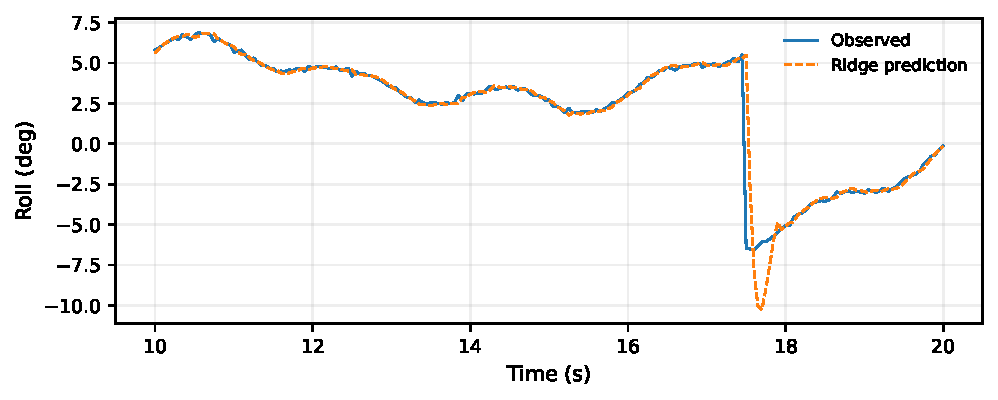
\includegraphics[width=.94\textwidth]{prediction.pdf}
\gzucaption{漂移区间附近的观测与预测}{Observed and predicted roll values near the drift interval}
\label{fig:prediction}
\end{figure}

\begin{figure}[htbp]
\centering
\begin{subfigure}{.48\textwidth}
  \centering
  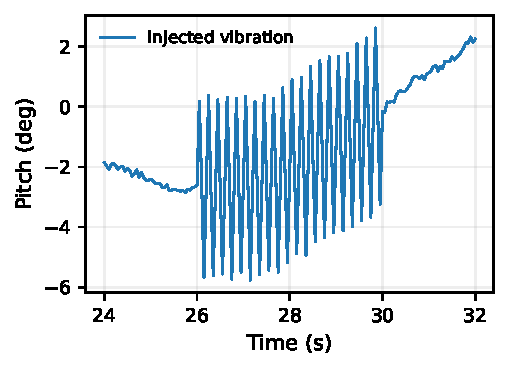
\includegraphics[width=\linewidth]{pitch-event.pdf}
  \caption{俯仰振动}\label{fig:pitch-sub}
\end{subfigure}\hfill
\begin{subfigure}{.48\textwidth}
  \centering
  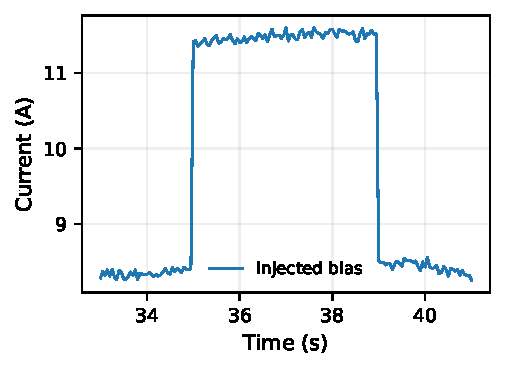
\includegraphics[width=\linewidth]{current-event.pdf}
  \caption{电流偏置}\label{fig:current-sub}
\end{subfigure}
\gzucaption{两类不同的合成异常片段}{Two different types of injected synthetic anomalies}
\label{fig:events}
\end{figure}

图~\ref{fig:events} 使用两个子图展示不同信号。
图~\ref{fig:events}\subref{fig:pitch-sub} 为高频振动，
图~\ref{fig:events}\subref{fig:current-sub} 为恒定偏置。
这一引用写法还用于检验子图编号与主图编号是否独立、稳定。
各子图的单独标题采用中文，图组总题注使用双语，未生成重复的插图清单条目。

\section{分数与平滑敏感性}
\begin{figure}[htbp]
\centering
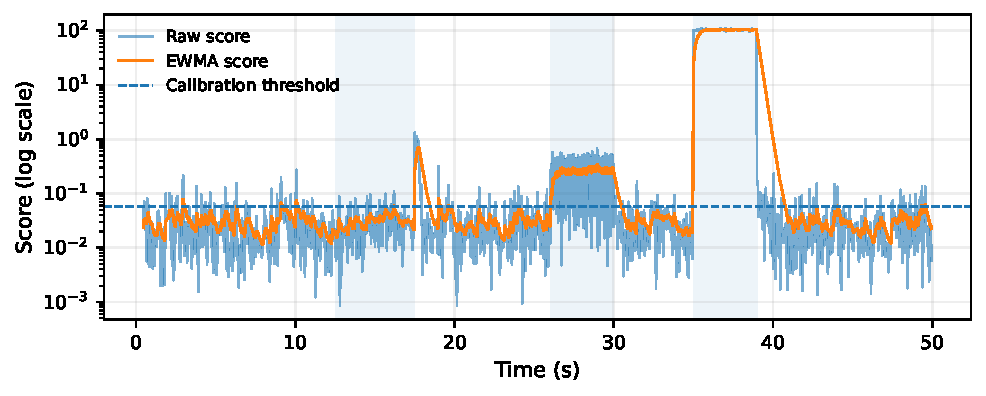
\includegraphics[width=.96\textwidth]{anomaly-score.pdf}
\gzucaption{原始残差、平滑分数与校准阈值}{Raw residuals, smoothed scores, and calibration threshold}
\label{fig:score}
\end{figure}

图~\ref{fig:score} 使用对数纵轴，同时绘出原始分数、平滑分数和固定阈值。
浅色区间表示生成器记录的异常位置，而不是模型预测。
平滑可以改变局部峰值，也会在异常结束后保留历史响应。
因此，在依赖持续观测的检测任务中，减少孤立峰值和增加响应延迟往往同时存在。

\begin{table}[htbp]
\centering
\gzucaption{平滑系数的敏感性分析}{Sensitivity analysis of the smoothing coefficient}
\label{tab:sensitivity}
\begin{tabular}{@{}rrrrr@{}}
\toprule
$\rho$ & P（\%） & R（\%） & F1（\%） & FAR（\%） \\
\midrule
\ExampleSensitivityRows
\bottomrule
\end{tabular}
\end{table}

\begin{figure}[htbp]
\centering
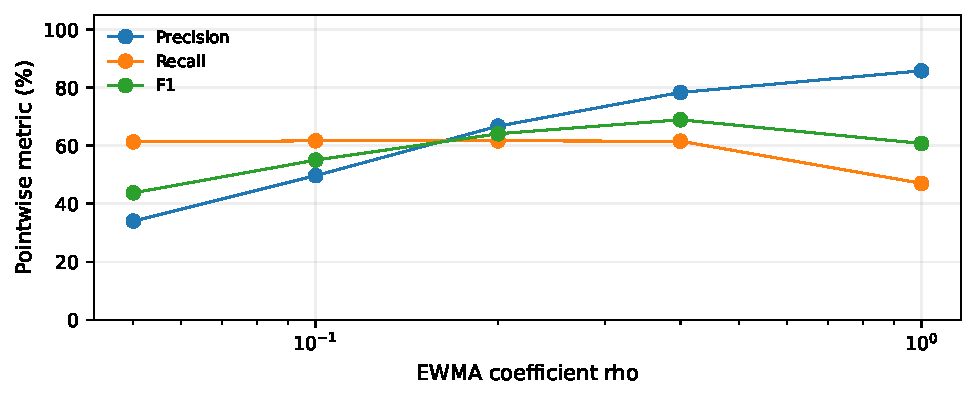
\includegraphics[width=.90\textwidth]{smoothing-sensitivity.pdf}
\gzucaption{不同平滑系数下的逐点指标}{Pointwise metrics under different smoothing coefficients}
\label{fig:sensitivity}
\end{figure}

表~\ref{tab:sensitivity} 和图~\ref{fig:sensitivity} 遍历预先指定的五个系数，
每个系数都重新使用校准数据估计阈值。本节是事后描述，不使用测试结果重新选定默认值。
若将该分析转换为正式模型选择，应再设置独立验证协议，而不能把测试集同时作为调参集。

\section{局限与结果解释}
首先，生成器只模拟少量连续信号与简单耦合，不包括传感器同步误差、
控制器闭环响应或真实故障的传播过程。其次，三次测试飞行共享同一类异常注入规则，
不能代表跨平台泛化。再次，没有重复运行多个随机种子，因而未报告均值和标准差。

最后，本文没有训练 LSTM、PatchTST、Anomaly Transformer 或 MOMENT。
这些模型仅在相关工作中被引用，不能将文献名称填入本例结果表并赋予虚构成绩。
需要比较这些方法时，应实现相同的数据协议、重新训练或按照公开模型的使用规则运行，
并在论文中区分原文结果、复现结果和本文结果。


% 参考文献
\bibliography{ref/refs}  % 参考文献使用 BibTeX 编译
% \printbibliography       % 参考文献使用 BibLaTeX 编译

% 附录
\appendix
\chapter{补充材料}
\label{app:extra}
附录编号和标题分别居中占一行。即使在后置部分命令之后，附录仍从 A 开始编号，页码则接续正文，不重新计数。
\section{附录公式}
如式~\eqref{eq:appendix}~所示，附录中的公式使用附录字母与序号组合编号。
\begin{equation}
  \sum_{i=1}^{n}(x_i-\bar{x})=0 .
  \label{eq:appendix}
\end{equation}


\chapter{补充实验}
\begin{gzuappendixrefs}

本附录引用了相关研究成果\cite{zhangkun1994}。
这里填写其他补充材料\cite{lin2013synthesis}。

% 附录独立参考文献
\gzuprintappendixbibliography{ref/refs}
\end{gzuappendixrefs}

\chapter{补充数据}
\begin{gzuappendixrefs}
本附录引用另一篇文献\cite{zhukezhen1973}。
\gzuprintappendixbibliography{ref/refs}
\end{gzuappendixrefs}



% 其他部分
\backmatter

% 致谢
% !TEX root = ../gzuthesis-example.tex

\begin{acknowledgements}
  衷心感谢导师×××教授和物理系××副教授对本人的精心指导。他们的言传身教将使我终生受益。

  在美国麻省理工学院化学系进行九个月的合作研究期间，承蒙 Robert Field 教授热心指导与帮助，不胜感激。

  感谢×××××实验室主任×××教授，以及实验室全体老师和同窗们学的热情帮助和支持！

  本课题承蒙国家自然科学基金资助，特此致谢。
\end{acknowledgements}


% 声明
% \statement
% 在提交终稿 PDF 时，先编译不含页眉页脚的声明页，以避免页码变化带来问题
% \statement[page-style=empty]
% 打印、签名、扫描为 PDF 文档后，将 scan-statement.pdf 替换原始页面，并生成页眉页脚
% \statement[file=scan-statement.pdf]

% 个人简历、在学期间完成的相关学术成果
% \input{data/resume}

% 指导教师/指导小组评语
% % !TEX root = ../gzuthesis-example.tex

\begin{comments}
% \begin{comments}[name = {指导小组评语}]
% \begin{comments}[name = {Comments from Thesis Supervisor}]
% \begin{comments}[name = {Comments from Thesis Supervision Committee}]

  论文提出了……

\end{comments}

% 答辩委员会决议书
% % !TEX root = ../gzuthesis-example.tex

\begin{resolution}

  论文提出了……

  论文取得的主要创新性成果包括：

  1. ……

  2. ……

  3. ……

  论文工作表明作者在×××××具有×××××知识，具有××××能力，论文××××，答辩××××。

  答辩委员会表决，（×票/一致）同意通过论文答辩，并建议授予×××（姓名）×××（门类）学博士/硕士学位。

\end{resolution}

\end{document}